% Requires \usepackage{graphicx} in the manuscript preamble.
% Paths are relative to the manuscript root.

\begin{figure}[htbp]
    \centering
    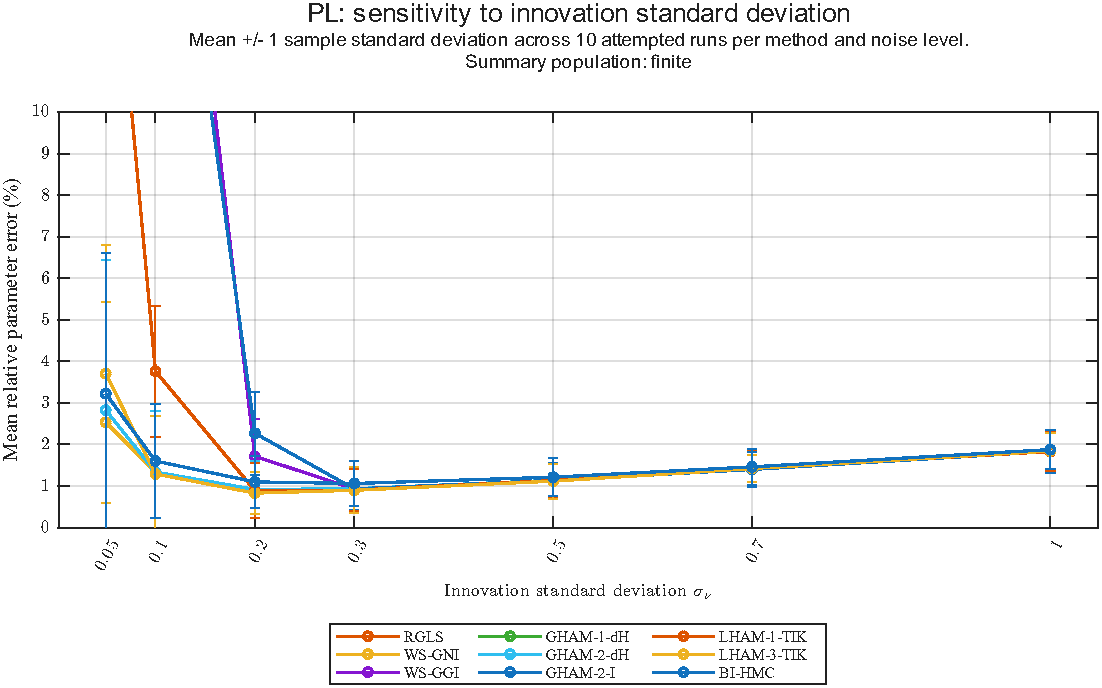
\includegraphics[width=\linewidth]
        {figs/noise_error_example_1_pl.pdf}
    \caption{Noise sensitivity for Example~1, PL comparison.
    Mean final relative parameter error; error bars indicate one sample
    standard deviation.
    Summaries retain valid finite outputs from ten attempted realizations
    per noise level.}
    \label{fig:noise_example_1_pl}
\end{figure}

\begin{figure}[htbp]
    \centering
    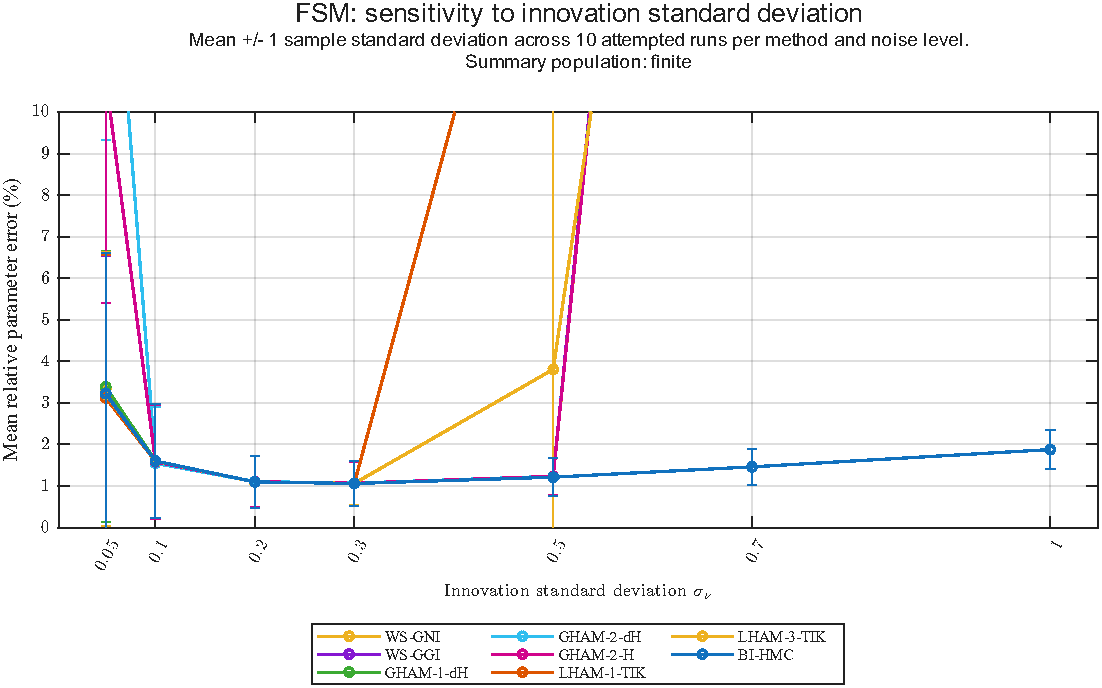
\includegraphics[width=\linewidth]
        {figs/noise_error_example_1_fsm.pdf}
    \caption{Noise sensitivity for Example~1, FSM comparison.
    Mean final relative parameter error; error bars indicate one sample
    standard deviation.
    Summaries retain valid finite outputs from ten attempted realizations
    per noise level.}
    \label{fig:noise_example_1_fsm}
\end{figure}

\begin{figure}[htbp]
    \centering
    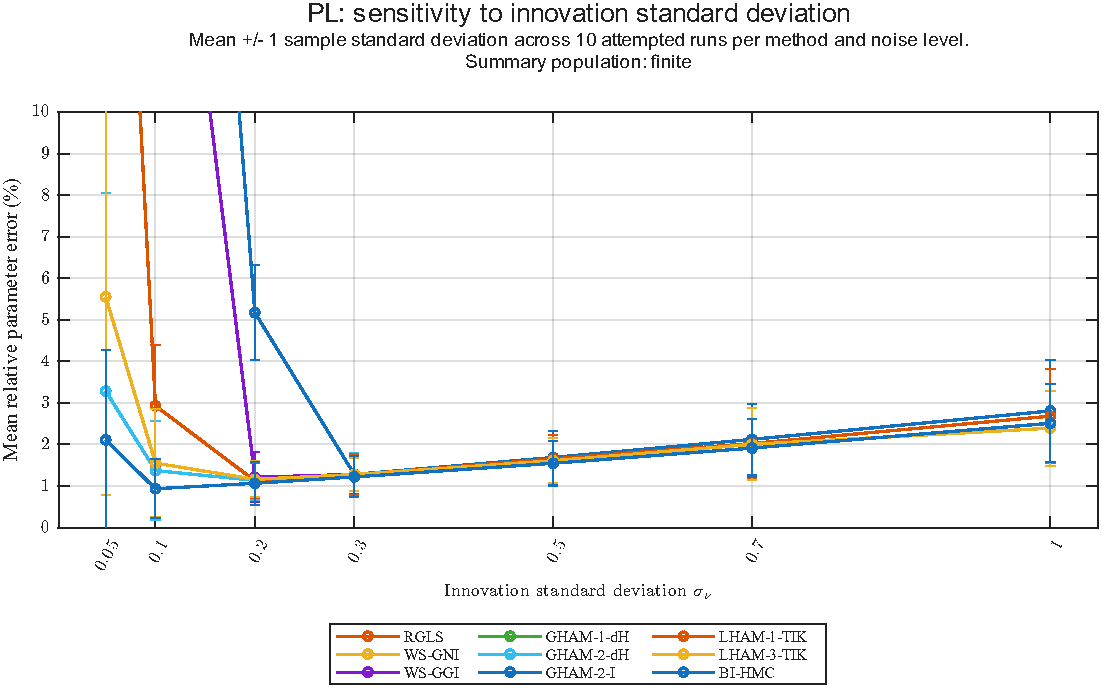
\includegraphics[width=\linewidth]
        {figs/noise_error_example_CSTR_pl.pdf}
    \caption{Noise sensitivity for CSTR, PL comparison.
    Mean final relative parameter error; error bars indicate one sample
    standard deviation.
    Summaries retain valid finite outputs from ten attempted realizations
    per noise level.}
    \label{fig:noise_example_cstr_pl}
\end{figure}

\begin{figure}[htbp]
    \centering
    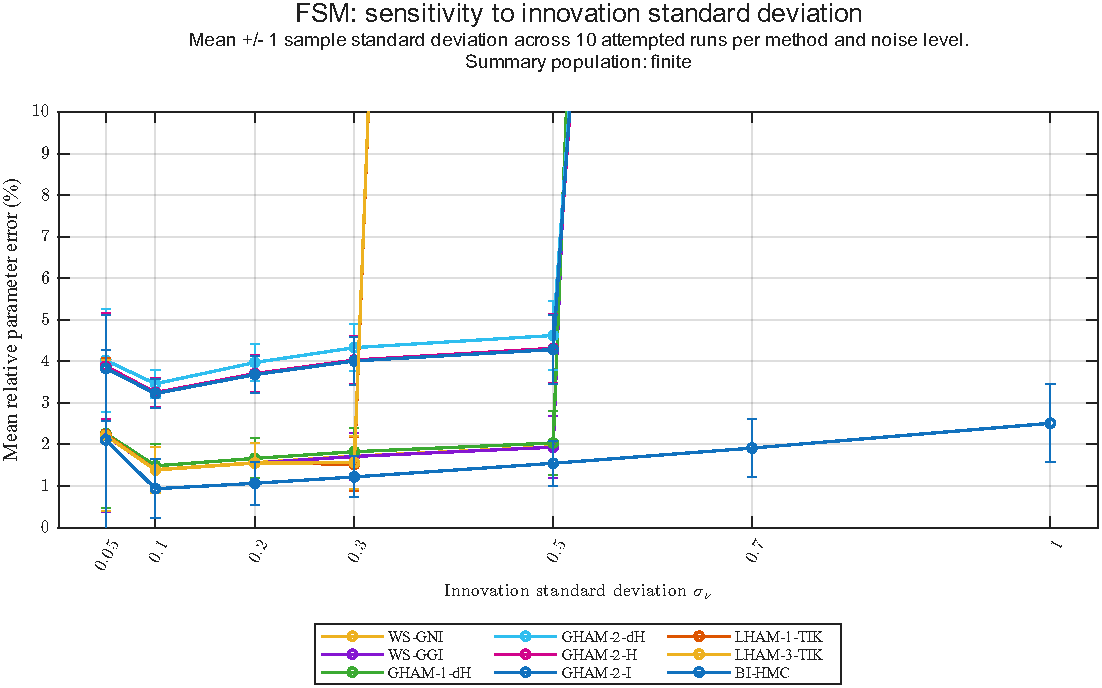
\includegraphics[width=\linewidth]
        {figs/noise_error_example_CSTR_fsm.pdf}
    \caption{Noise sensitivity for CSTR, FSM comparison.
    Mean final relative parameter error; error bars indicate one sample
    standard deviation.
    Summaries retain valid finite outputs from ten attempted realizations
    per noise level.}
    \label{fig:noise_example_cstr_fsm}
\end{figure}

